\documentclass[platz]{tudphygp}
\usepackage{tudphymd}

\versuch{Fehleranalyse}{FA}
\author{Dr. Tirschler }
\date{01.03.2007}

\begin{document}
\maketitle

\section*{Aufgabenstellung}

Bestimmen Sie die Schwingungsdauer eines Fadenpendels $T$ in \num{10} bis \num{200} Einzelmessungen, und analysieren Sie die Resultate hinsichtlich des arithmetischen Mittels $\overline T$, der Standardabweichung $s_T$ und der Verteilungsfunktion von $T$:
\begin{enumerate}
 \item F�r \num{10} Einzelmessungen sind von Hand $\overline T$ und $s_T$ zu berechnen.
 \item Nach der Klasseneinteilung werden \num{200} Messungen durchgef�hrt und mit dem zur Verf�gung stehenden Programm ausgewertet. Dabei werden nach \num{10}, \num{25}, \num{50}, \num{100} und \num{200} die H�ufigkeiten der Messwerte ermittelt, woran die Entwicklung der Statistik beobachtet werden kann.
 \item Aus den gewonnenen Daten ist die Fallbeschleunigung $g$ samt Fehler zu bestimmen.
 \item \emph{(F�r Physikstudenten)} F�r die einzelnen Messungen ist anhand der H�ufigkeitsverteilung und einer Darstellung der Summenkurve auf Wahrscheinlichkeitspapier das Vorliegen einer Gau�-Verteilung zu pr�fen.
\end{enumerate}

\section*{Hinweise zur Versuchsdurchf�hrung}

\begin{itemize}
 \item Um den subjektiven Einfluss zu erh�hen, stoppen Sie $T$ am Umkehrpunkt des Pendels.
 \item Die Amplitude der Pendelschwingung sollte \SI{15}{cm} nicht �berschreiten. Die Messreihe im Programmteil "`Starten"' kann unterbrochen werden, um das Pendel neu anzuregen, wenn sich durch verschiedene �u�ere Einfl�sse eine elliptische Schwingung einstellen sollte.
\end{itemize}
Die Datenerfassung und -auswertung erfolgt durch ein Excel-Programm. Zahlen sind nach englischer Notation mit Komma (nicht mit Punkt!) einzugeben. Die einzelnen Programmschritte (siehe auch Abb.~\ref{fig::interface}) sind nacheinander auszuf�hren.
\par\textbf{Achtung:} Geben Sie bei Kontrollabfragen $>4$ falsche Ergebnisse ein, wird der Versuch nicht anerkannt.
\begin{itemize}
 \item Beim Vorversuch m�ssen Sie alle Einzelmessungen ins Protokoll �bernehmen und die statistischen Kenngr��en wie den Mittelwert und die Standardabweichungen der Einzelmessungen und des Mittelwertes berechnen. Ihre Auswertungen werden kontrolliert.
 \item F�r die Festlegung der Intervalleinteilung nutzen Sie die Ergebnisse des Vorversuches. Empfohlen wird eine Intervalleinteilung, bei der \SI{99,9}\% der Messwerte innerhalb der Intervalleinteilung liegen (Messintervalle von $T - 3\sigma$ bis $T + 3\sigma$).
 \item Die Erfassung, Auswertung und Darstellung der Messwerte des Hauptversuches erfolgen durch den Computer. F�r das Protokoll stellen Sie aus Tabellen und Diagrammen eine Druckseite f�r Ihr Protokoll zusammen, die wichtige statistische Ergebnisse des Versuches veranschaulicht. Nutzen Sie auch die M�glichkeit, Variationen in der Anzahl der auszuwertende Messwerte und der Intervalleinteilung vorzunehmen (Men�punkt: "`Pr�fung Normalverteilung"').
 \item Bevor Sie den Programmpunkt "`$g$-Ermittlung"' starten, erfassen Sie alle daf�r ben�tigten Gr��en einschlie�lich ihrer Fehler im Protokoll und berechnen die Fallbeschleunigung $g$ und deren Fehler $\Delta g$. Beim Programmpunkt "`$g$-Ermittlung"' wird gepr�ft, ob Sie die korrekten Gr��en erfasst und die Fallbeschleunigung $g$ einschlie�lich Fehler richtig berechnet haben.
 \item Im Protokoll ist auch das Endergebnis in der Form $g = \kla{\ldots \pm \ldots \pm \ldots}{\frac m{s^2}}$ (Physiker geben systematische und statistische Messunsicherheit getrennt an) bzw. $g = \errSI{\ldots}{\ldots}{\frac m{s^2}}$ (Ingenieure) herauszustellen. In der Diskussion sollten Sie auf beide Teile des Versuches (Statistik; $g$-Ermittlung) kurz eingehen.
\end{itemize}

\begin{figure}[h!]
 \centering
 \fbox{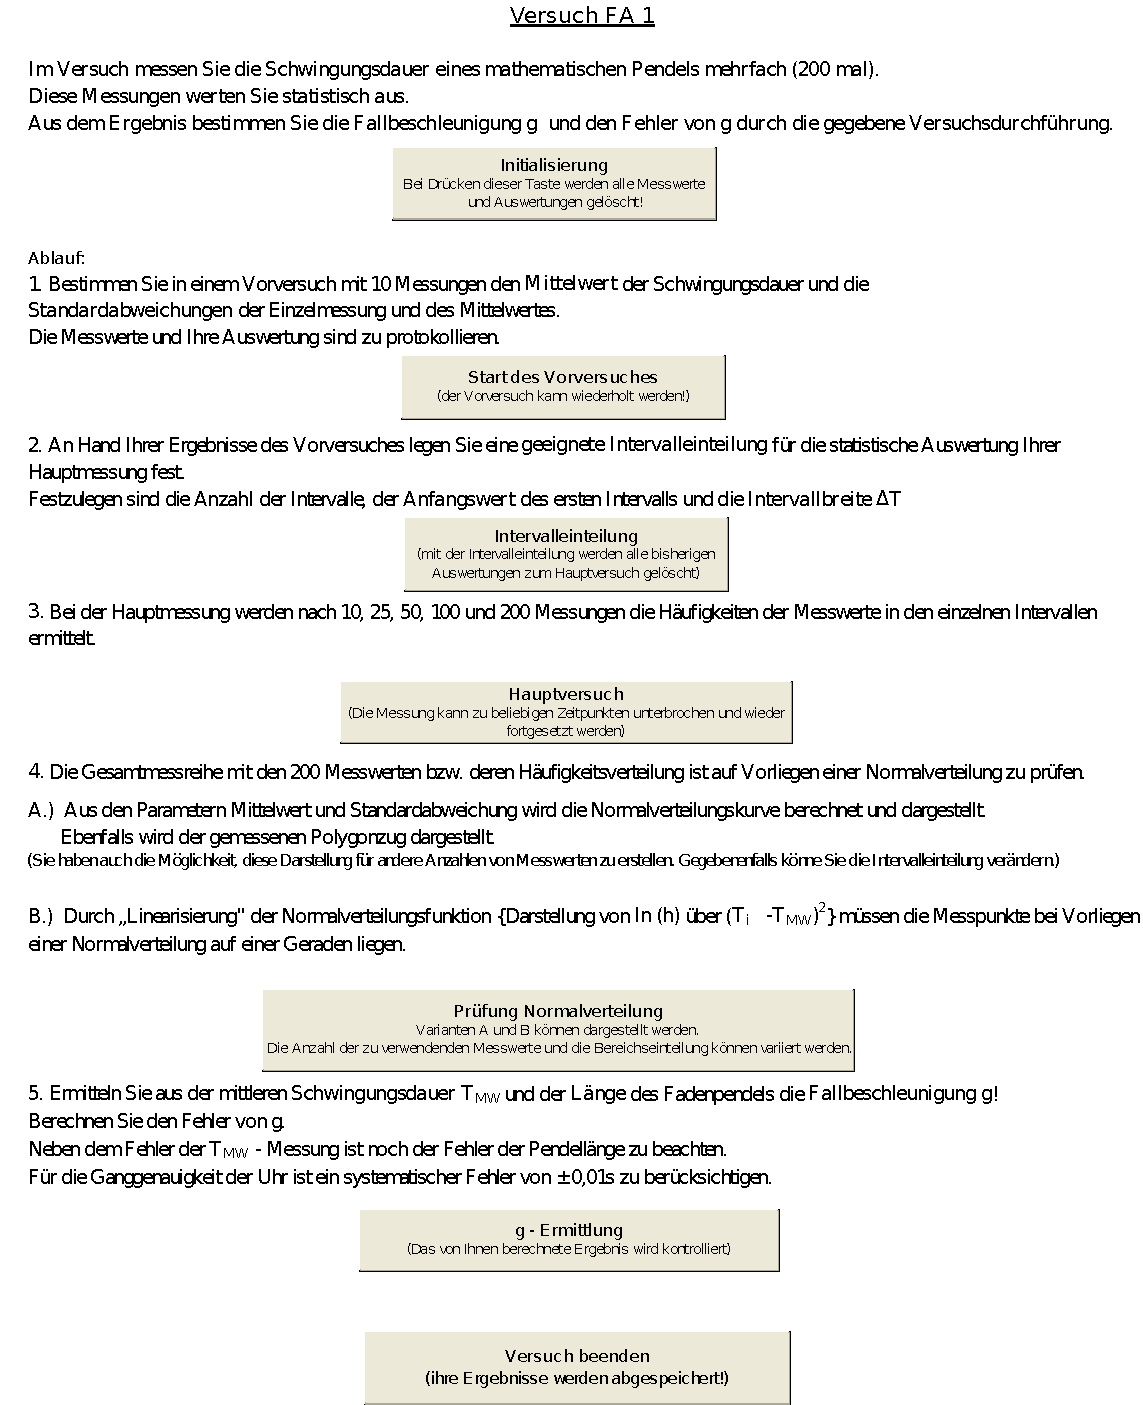
\includegraphics[width=\linewidth]{GP1-FA-Interface.pdf}}
 \caption{�bersicht �ber die Startseite des Computerprogramms mit den einzelnen
 Programmschritten \label{fig::interface}}
\end{figure}


\end{document}
